\documentclass[a4paper, 9pt]{article}

\usepackage{amsmath}
\usepackage{amssymb}
\usepackage{graphicx}
\graphicspath{ {./images/} }
\usepackage{rotating}
\usepackage{float}

\usepackage[a4paper,
            left=0.6in,
            right=0.6in,
            top=1in,
            bottom=1in]{geometry}

\usepackage{hyperref}
\usepackage{lipsum}

\usepackage{multicol}
\setlength{\columnsep}{0.4cm}

\title{Application of High Dimensional Techniques to House Price Prediction}
\vspace{5pt}

\author{
  Pala, Alessandro\\
  \texttt{alessandro.pala@studenti.unipd.it}
  \and
  Tremaggi, Domenico\\
  \texttt{domenico.tremaggi@studenti.unipd.it}
}
\date{}

\begin{document}

\maketitle
\noindent
\begin{abstract}
 This study explores the use of linear regression, lasso regression, group lasso regression, and a simple neural network to predict house prices based on various features, such as location, size, and the number of rooms. The primary goal is to assess the performance of these models in terms of predictive accuracy, feature selection, and their ability to handle multicollinearity in the dataset.
\end{abstract}
\vspace{5pt}

\begin{multicols}{2}

\section{Introduction} \vspace{-7pt}
In order to approach the dataset, we first think about which models and variables can predict real estate prices in the real world, with the constraint of the set of variables given by the dataset. Since we handle a price prediction regression, a fair comparison of linear and non-linear basic models - be them regularized or not - would be multivariate. Hence, we first carry a synthetic application of the following models: multivariate linear model and multivariate Poisson regression with an $\alpha = 0.1$ Elastic Net.

We then train a deep Multi-Layer Perceptron for performance comparison and we regularize it with a simple Lasso.
Finally, we utilise a Group Lasso regression on two sets of groups of variables that we think may be good predictors of house prices in the real world. The first set of groups uses variables that are usually clustered together by real estate professionals when they do house price estimation. The second set of groups uses clusters of highly statistically correlated (Pearson's $r$) variables.(Figure \ref{fig:corrmatplot})

All selection for regularized models is carried through with cross-validation.

\section{Dataset} \vspace{-7pt}
The dataset contains real estate property listings, each described by a variety of attributes. Temporal attributes are: the listing date, the year the property was built, and the year of its last renovation. Physical characteristics are: the number of bedrooms and bathrooms, living area size, total lot size, number of floors, basement area, and living area above ground. Scenic qualities are represented by a waterfront view indicator, a view quality rating, an overall condition rating, and an overall grade rating. Locational data instead include zip code,  latitude, and longitude. There is also some additional spatial context given by the average living area and lot sizes of the 15 nearest properties.

\subsection{Pre-processing} \vspace{-3pt}
In order to pre-process the data, we first convert the date column into a proper date object by extracting the first 8 characters (in "YYYYMMDD" format). We then replace 0 values in the "yr{\_}renovated" column with NA, treating them as missing data. Duplicate rows are removed based on the id column.
We add new variables in the dataset: total{\_}sqft calculates total area by summing living and basement space, bath{\_}per{\_}bed computes the bathroom-to-bedroom ratio (defaulting to 0 if bedrooms are 0), and total{\_}rooms sums bedrooms and bathrooms. sqft{\_}diff{\_}15 measures the difference between the property’s living area and that of its 15 nearest neighbors, while age{\_}since{\_}reno calculates the property’s age since construction, defaulting to 0 if the year is invalid. (Figure \ref{fig:corrplots})
The first, second, fifteenth and sixteenth columns are dropped since they are analytically irrelevant (date, id, with yr{\_}built and yr{\_}renovated being substituted by "age"). We then scale the features of the data frame.
The price and the non-structural features are extracted as columns 2 to 18 and scaled in the new matrix X, which will be used for the Group Lasso. The price, or target, is stored in a separate vector Y.

\section{Base Models} \vspace{-7pt}
\subsection{Multivariate linear model} \vspace{-3pt}
Multivariate Linear Regression is an extension of linear regression where the goal is to model the relationship between multiple independent variables (also called predictors or features) and a dependent variable (also called the target or response variable). It is used when you have more than one predictor variable that you believe influences the dependent variable.

\subsubsection*{Mathematical equation}
\begin{equation}
Y=\beta_0+\beta_1X_1+\beta_2X_2+\dots+\beta_kX_k+\epsilon
\end{equation}

where:$Y$ is the dependent variable, ($X_1, X_2,\dots,X_k$) are the independent variables, $\beta_0$ is the intercept, ($\beta_1,\beta_2, \dots, \beta_k$) are the coefficients and $\epsilon$ is the error term.\\
\subsubsection*{Experiments}
In our case of interest we use all the the available variables to estimate the house prices(Table \ref{tab:mlrcoeffs})(Figure \ref{fig:MLR}).\\
Among our predictors we find that only the intercept and the coefficient for bedrooms are statistically significant at the 0.001 level, with p-values less than 2e-16. Other predictors like bathrooms, sqft$\_$living, and sqft{\_}lot have high p-values, hence not statistically significant. The zipcode has been omitted because of singularity, meaning either multicollinearity or redundancy. The residual standard error of the model at 6.15e-09 is very low and in general the residuals are also very small, ranging from -7.36e-07 to 1.38e-09. The F-statistic is astronomically large at 4.788e+30.\\
This multivariate regression is "perfect", given that the adjusted R-squared values are 1, with predictors explaining all the variability in the response variable. This is clearly a case of overfitting, which we need to handle with regularization. \ref{fig:corrplots}


\subsection{Multivariate GLM with Elastic Net} \vspace{-3pt}
\subsubsection*{The Poisson Distribution}
Poisson regression is based on the Poisson distribution, which describes the probability of a given number of events occurring in a fixed interval of time or space, given the average rate of occurrence.\\
The probability mass function of a Poisson-distributed random variable $Y$ is:
\begin{equation}
P(Y=y)= \frac{\lambda^ye^{-\lambda}}{y!}
\end{equation}
Where: $y$ is the count of events (e.g., number of accidents, number of emails received) and $\lambda$ is the rate of occurrence, which is the expected number of events in the fixed interval.
\subsubsection*{The Poisson Regression Model}
Poisson regression assumes that the logarithm of the expected count (rate) is a linear function of the independent variables.\\
The model is expressed as:
\begin{equation}
\log(\lambda_i)=\beta_0+\beta_1X_1+\beta_2X_2+\dots+\beta_kX_k
\end{equation}
where: ($X_1, X_2,\dots,X_k$) are the indipendent variables, $\beta_0$ is the intercept, ($\beta_1,\beta_2, \dots, \beta_k$) are the regression coefficients
\subsubsection*{Elastic Net}
In regular linear regression or GLMs, the model can overfit the data if there are many predictors, especially when some predictors are irrelevant or highly correlated, but it can also use some sparsity enforcement, so we applied an Elastic Net regression. This kind of regularization combines $L_1$ and $L_2$ regularizations and applies penalty to coefficients as to: 
\begin{itemize}
\item Lasso ($L_1$1): Shrink some coefficients to zero, performing feature selection.(Figure \ref{fig:MGLM})
\item Ridge ($L_2$): Shrink the coefficients (but not set them to zero) helping with multicollinearity, which our dataset suffers from.
\end{itemize}
Mathematically, the Elastic Net penalty is given by:
\begin{equation}
\text{Penalty}= \gamma \left[\alpha \sum_{j=1}^k|\beta_j| + \frac{1}{2}(1-\alpha)\sum_{j=1}^k\beta_{j}^{2} \right]
\end{equation} 
where $\gamma$ controls the strength of the regularization (larger $\gamma$ means more regularization), $\alpha$ controls the balance between Lasso and Ridge. If $\alpha=1$, the penalty is purely Lasso; if $\alpha=0$, the penalty is purely Ridge, meaning our $\alpha = 0.1$ choice mostly applies an $L_2$ penalty. We chose this hyperparameter after some experiments that suggested that even a very small Lasso penalty enforced sparsity efficiently.
\subsubsection*{Poisson Regression with Elastic Net}
When you combine Poisson regression with Elastic Net regularization the model becomes:
\begin{equation}
\begin{split}
\log(\lambda_i)&=\beta_0+\beta_1X_1+\beta_2X_2+\dots+\beta_kX_k+ \\
&+\gamma \left[\alpha \sum_{j=1}^k|\beta_j| + \frac{1}{2}(1-\alpha)\sum_{j=1}^k\beta_{j}^{2} \right]
\end{split}
\end{equation}
This means that the objective is to minimize the following loss function:
\begin{equation*}
\text{Loss}=\sum_{i=1}^n(-Y_i \log(\lambda_i)+ \lambda_i)+ \gamma \left[\alpha \sum_{j=1}^k|\beta_j| + \frac{1}{2}(1-\alpha)\sum_{j=1}^k\beta_{j}^{2} \right]
\end{equation*}

\subsubsection*{Experiments}
The Poisson regression model(Table \ref{tab:glmcoeffs})output shows that the intercept is 540,529.7, which means that when all the predictors are zero, the dependent variable has a high baseline value. The coefficient for Bedrooms is 356,970.6, which means that with every additional bedroom, the expected value of the outcome increases significantly, holding other factors constant. However, many other factors like Bathrooms, Sqft$\_$Living, Sqft$\_$Lot, Floors, etc., have missing coefficients, represented by periods, and most likely because these variables were excluded from the model, had no significant relationship with the result(Figure \ref{fig:MGLMcv}). A simple analysis of actual target values compared to predicted values shows that the model is very successful at predicting while not overfitting the data since the presence of Elastic Net regularization.(Figure \ref{fig:MGLMpred})

\section{Group Lasso} \vspace{-7pt}
The Group Lasso is an extension of the classical Lasso method applied for regularization and variable selection designed to work with grouped variables, and such a situation is helpful when given variables naturally fall into groups, and we want to choose or discard entire groups of variables simultaneously rather than choosing or dropping individual variables.

The main mathematical goal of the Group Lasso is to do regression by penalizing the sum of the norms of the coefficients in each group. That will induce sparsity at the level of groups, that is, all coefficients in a group will either be shrunk towards zero, or not. Therefore, entire groups of variables are either selected or not.

\subsection{Mathematical Formulation} \vspace{-3pt}
For a given linear regression problem, the model can be represented as:
\begin{equation}
y=X\beta + \epsilon
\end{equation}
where: $y$ is the $n \times 1$ vector of observed responses, $X$ is the $n \times p$ matrix of predictors, $\beta$ is the $p \times 1$ vector of regression coefficient and $\epsilon$ is the error term, assumed to be normally distributed.\\

In ordinary linear regression, we try to minimize the residual squared error: \begin{equation} \min_{\beta}\left (\frac{1}{2n}\lVert y-X\beta\rVert^{2}_{2} \right) 
\end{equation}

In the case of Group Lasso, we add a regularization term to the objective function that penalizes the coefficients in groups. If the variables are divided into $G$ groups, and group $g$ contains $p_{g}$ variables, the Group Lasso penalty is given by: \begin{equation} \lambda \sum_{g=1}^{G}\lVert \beta_{g} \rVert_{2}
\end{equation}

The idea would be: where: $\beta_g$ represents the coefficient corresponding to the $g$-th group of variables, $\lVert \beta_g \rVert_2$ is the euclidean norm of the coefficient vector, $\lambda$ is a regularization parameter that regulates its strength.

Thus, the optimization problem is: \begin{equation}
\min_{\beta}\left (\frac{1}{2n}\lVert y-X\beta\rVert^{2}_{2} + \lambda \sum_{g=1}^{G}\lVert \beta_{g} \rVert_{2}\right)
\end{equation}

\subsection{Experiments} \vspace{-3pt}

Anyway, even with this more complex model, the most important variables predicting the prices were the same as before, surely some minor correlation rise up, but not so strong to be considered meaningful for our purposes. (Figure \ref{fig:gglassocoefpath})(Figure \ref{fig:gglassoheat})(Figure \ref{fig:gglassocv})(Figure \ref{fig:gglassofeatures})(Figure \ref{fig:gglassocverror})(Figure \ref{fig:gglasso1pred})(Figure \ref{fig:gglasso2pred})

\section{Neural Network} \vspace{-7pt}
We finally train a deep neural network in order to check which could be the best possible result in any statistical context and if our model choice was insufficient.\\
The architecture is kept neither too deep nor too shallow given the medium number of features. We see very clearly that the network can use the features of the dataset to predict extremely well. The goal of this small experiment was to satiate any doubt about the dataset being corrupted, and that any model could somehow suffer from problems. Indeed, the dataset is not corrupted, but simply seems to (counterintuitively, with respect to the context) present only one feature out of many with actual predictive power.(Figure \ref{fig:NNpred})(Figure \ref{fig:NN})(Figure \ref{fig:traintestloss})(Table \ref{tab:nn})

\section{Conclusion} \vspace{-7pt}
\noindent

\end{multicols}


\pagebreak
\appendix

\section{Visualization}
\begin{figure}[h]
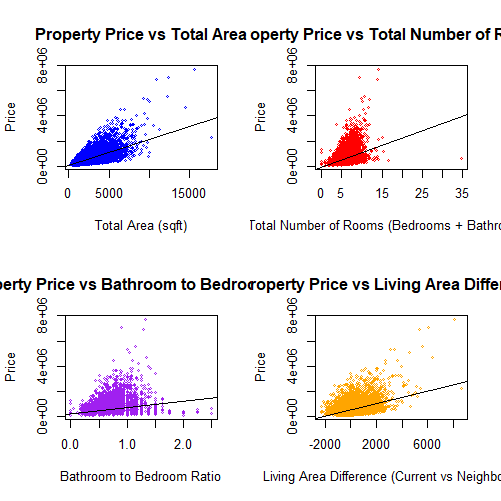
\includegraphics[scale=0.6]{corrplots}
\centering
\caption{How price behaves with aggregated variables}
\label{fig:corrplots}
\end{figure}

\begin{figure}[H]
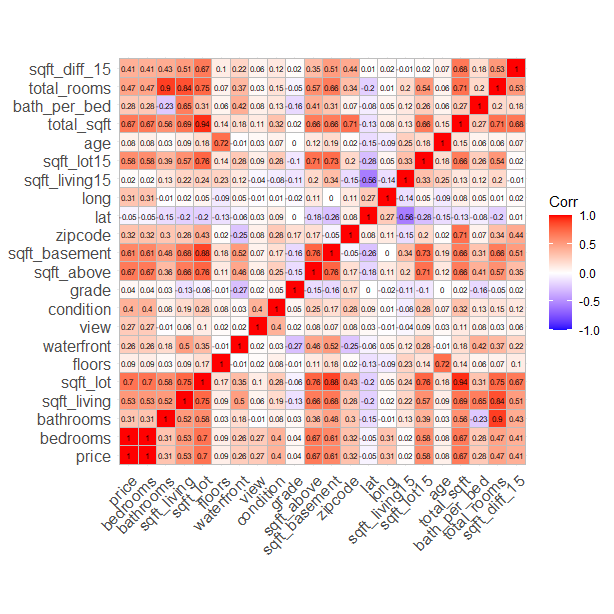
\includegraphics[scale=0.8]{corrmatplot}
\centering
\caption{Correlation matrix to pick groups in the second set of Group Lasso}
\label{fig:corrmatplot}
\end{figure}


\section{Regressions}
\begin{figure}[H]
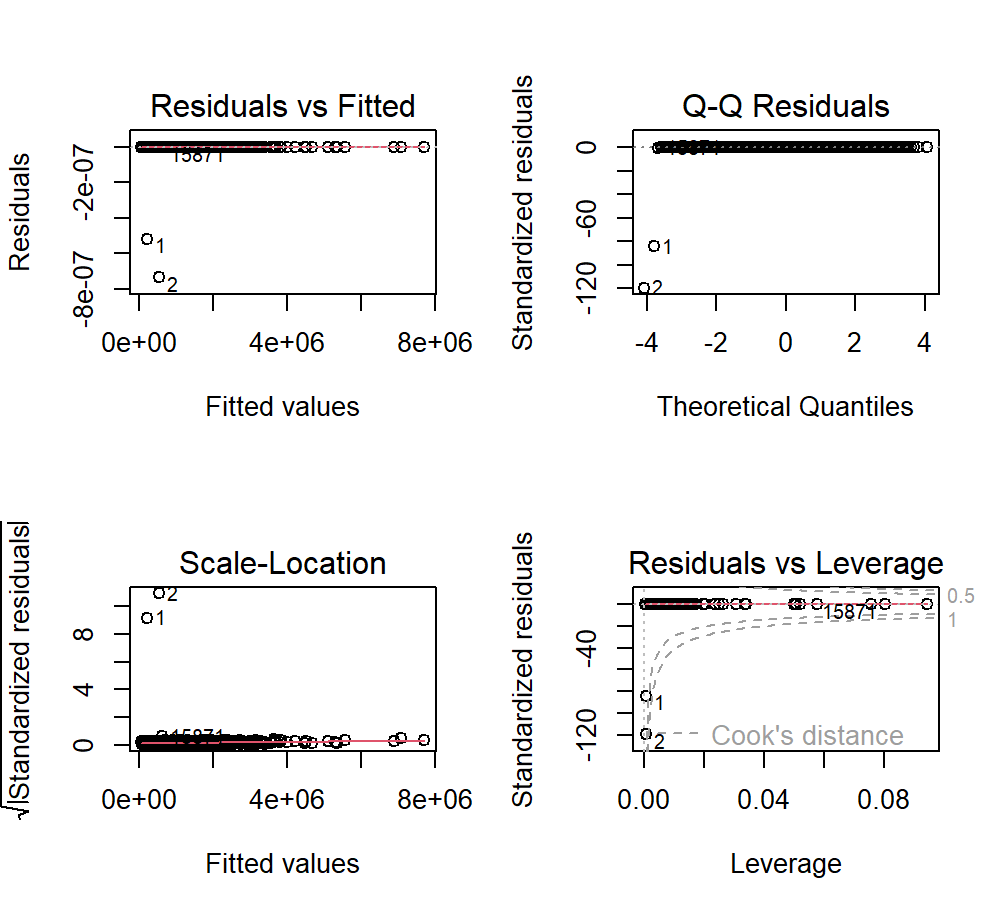
\includegraphics[scale=0.9]{MLR}
\centering
\caption{Multivariate linear regression plot}
\label{fig:MLR}
\end{figure}

\begin{table}[ht]
\centering
\begin{tabular}{|l|r|r|r|r|}
\hline
\textbf{Variable} & \textbf{Estimate} & \textbf{Std. Error} & \textbf{t value} & \textbf{p value} \\
\hline
(Intercept)       & 5.405e+05   & 4.201e-11  & 1.287e+16  & $<$ 2e-16 ***  \\
bedrooms          & 3.677e+05   & 7.398e-11  & 4.970e+15  & $<$ 2e-16 ***  \\
bathrooms         & 7.485e-11   & 5.423e-11  & 1.380e+00  & 0.168        \\
sqft$\_$living       & 3.946e-11   & 7.260e-11  & 5.440e-01  & 0.587        \\
sqft$\_$lot          & -1.557e-10  & 1.267e-10  & -1.229e+00 & 0.219        \\
floors            & 7.671e-12   & 6.084e-11  & 1.260e-01  & 0.900        \\
waterfront        & -1.241e-11  & 5.815e-11  & -2.130e-01 & 0.831        \\
view              & -6.033e-12  & 4.719e-11  & -1.280e-01 & 0.898        \\
condition         & 1.576e-11   & 5.097e-11  & 3.090e-01  & 0.757        \\
grade             & 3.389e-11   & 4.487e-11  & 7.550e-01  & 0.450        \\
sqft$\_$above        & 7.269e-11   & 7.782e-11  & 9.340e-01  & 0.350        \\
sqft$\_$basement     & -4.531e-11  & 1.110e-10  & -4.080e-01 & 0.683        \\
zipcode           & NA          & NA         & NA         & NA           \\
lat               & -6.270e-11  & 5.391e-11  & -1.163e+00 & 0.245        \\
long              & -2.108e-11  & 4.867e-11  & -4.330e-01 & 0.665        \\
sqft$\_$living15     & -1.568e-13  & 5.590e-11  & -3.000e-03 & 0.998        \\
sqft$\_$lot15        & 5.429e-11   & 7.241e-11  & 7.500e-01  & 0.453        \\
age               & 5.543e-12   & 6.138e-11  & 9.000e-02  & 0.928        \\
\hline
\end{tabular}
\caption{Multivariate Linear Regression Data Summary}
\label{tab:mlrcoeffs}
\end{table}


\begin{figure}[H]
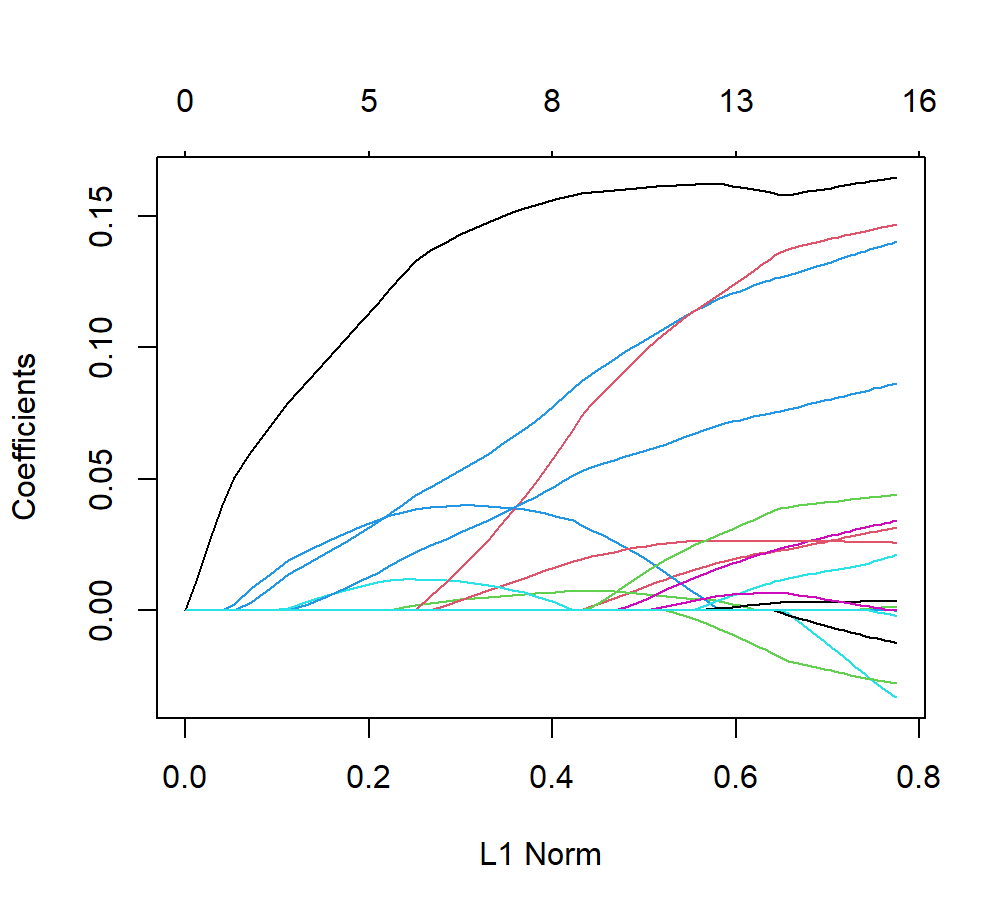
\includegraphics[scale=0.9]{MGLM}
\centering
\caption{Multivariate Poisson regression coefficient path}
\label{fig:MGLM}
\end{figure}

\begin{figure}[H]
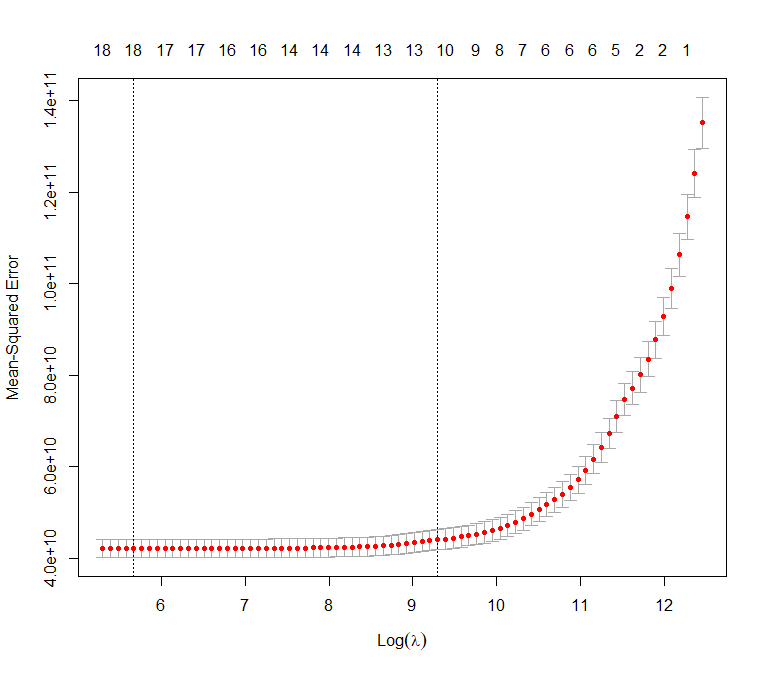
\includegraphics[scale=0.8]{MGLMcv}
\centering
\caption{Cross validation plot for Poisson regression}
\label{fig:MGLMcv}
\end{figure}


\begin{table}[ht]
\centering
\begin{tabular}{|l | r|}
\hline
\textbf{Variable} & \textbf{Coefficient} \\
\hline
Intercept     & 540529.7 \\
Bedrooms      & 356970.6 \\
Bathrooms     & . \\
Sqft\_Living   & . \\
Sqft\_Lot      & . \\
Floors        & . \\
Waterfront    & . \\
View          & . \\
Condition     & . \\
Grade         & . \\
Sqft\_Above    & . \\
Sqft\_Basement & . \\
Zipcode       & . \\
Lat           & . \\
Long          & . \\
Sqft\_Living15 & . \\
Sqft\_Lot15    & . \\
Age           & . \\
\hline
\end{tabular}
\caption{Coefficients from the Poisson model}
\label{tab:glmcoefs}
\end{table}

\begin{figure}[H]
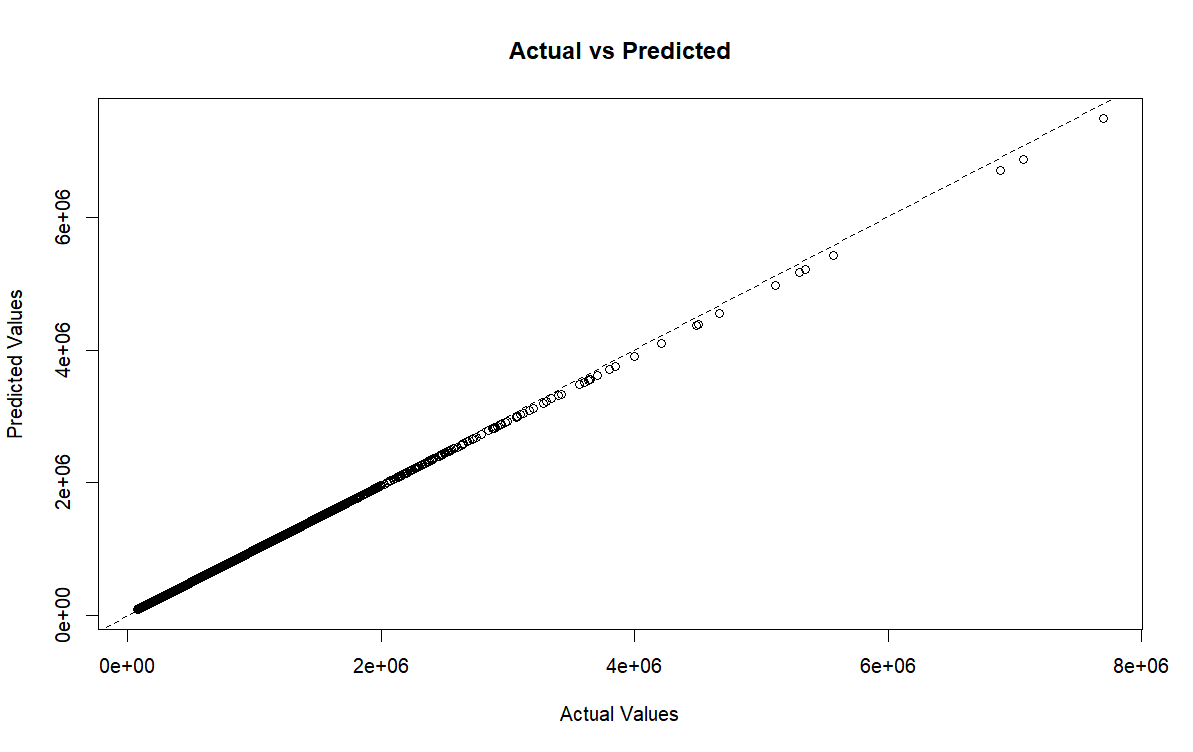
\includegraphics[scale=0.65]{MGLMpred}
\centering
\caption{Poisson regression actual vs predicted}
\label{fig:MGLMpred}
\end{figure}

\begin{figure}[H]
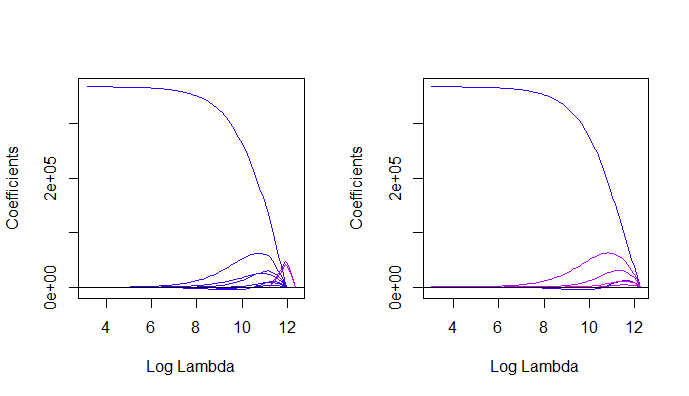
\includegraphics[scale=0.9]{gglassobasic}
\centering
\caption{Group sets comparison for Group Lasso}
\label{fig:MGLMpred}
\end{figure}

\begin{figure}[H]
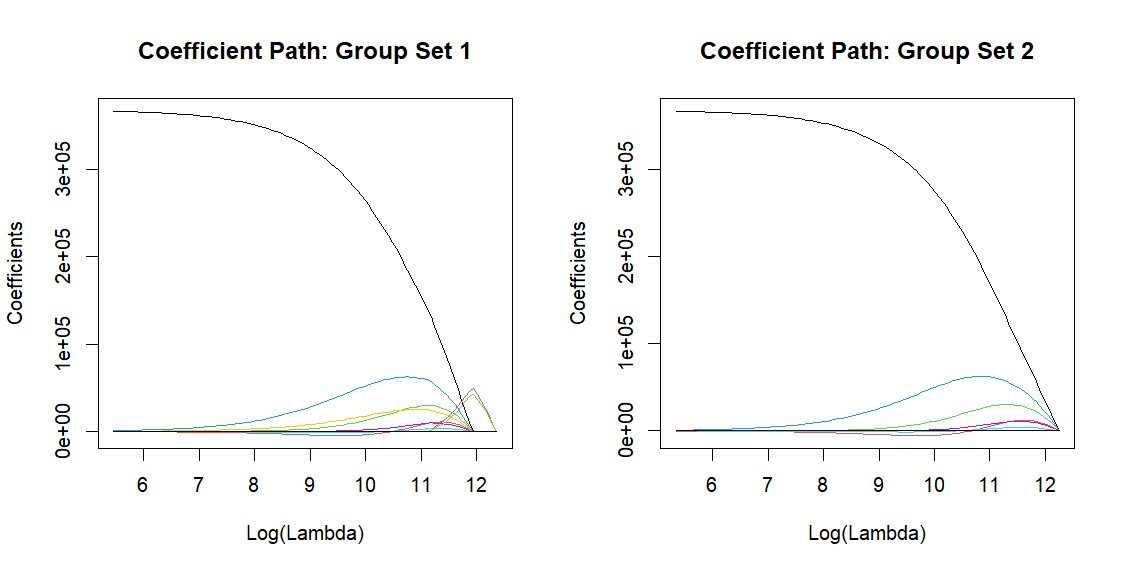
\includegraphics[scale=0.7]{gglassocoefpath}
\centering
\caption{Coefficient path for Group Lasso}
\label{fig:gglassocoefpath}
\end{figure}

\begin{figure}[H]
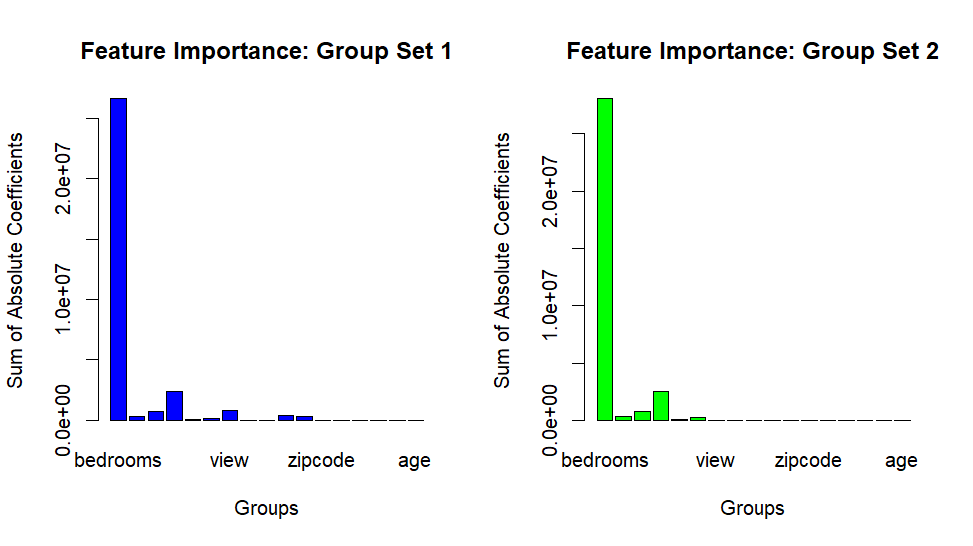
\includegraphics[scale=0.8]{gglassofeatures}
\centering
\caption{Best features for each group set for Group Lasso}
\label{fig:gglassofeatures}
\end{figure}

\begin{figure}[H]
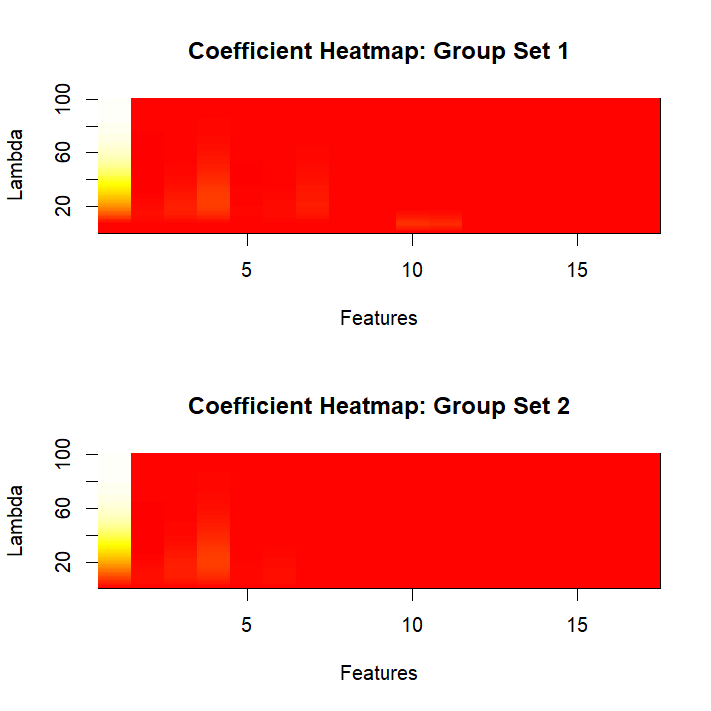
\includegraphics[scale=0.8]{gglassoheat}
\centering
\caption{Feature heatmap for Group Lasso}
\label{fig:gglassoheat}
\end{figure}

\begin{figure}[H]
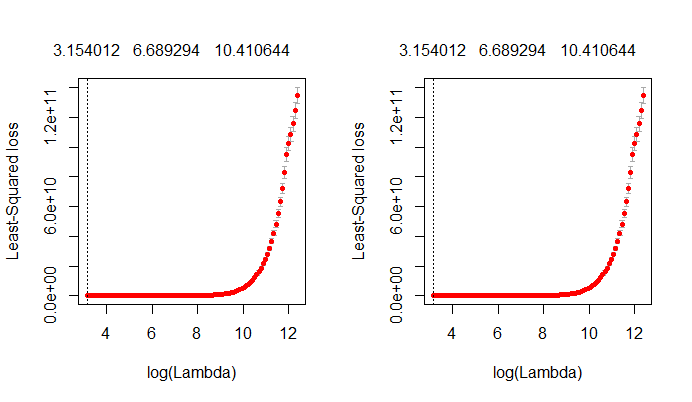
\includegraphics[scale=0.85]{gglassocv}
\centering
\caption{Cross validation plot for Group Lasso}
\label{fig:gglassocv}

\end{figure}

\begin{figure}[H]
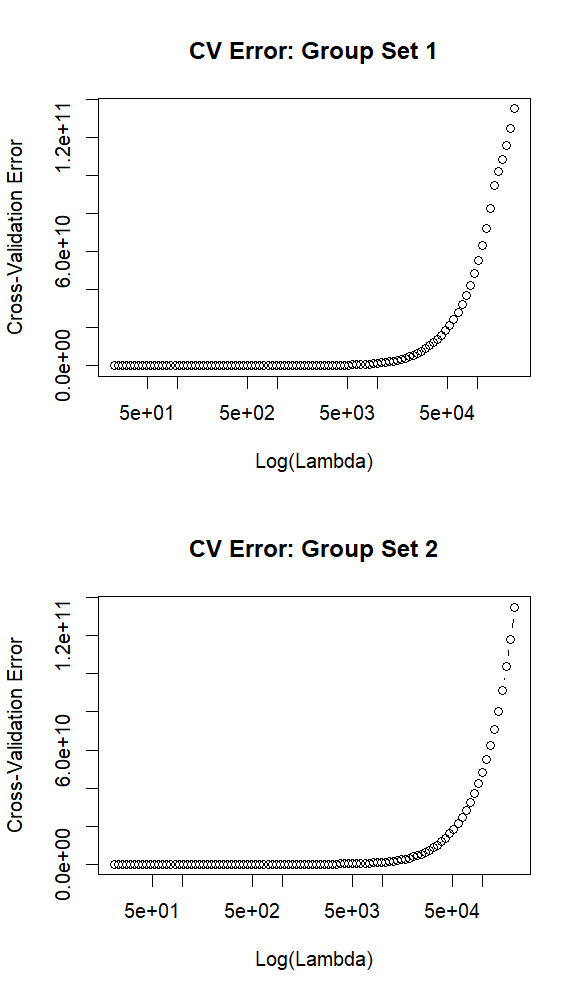
\includegraphics[scale=0.85]{gglassocverror}
\centering
\caption{Cross validation error for Group Lasso}
\label{fig:gglassocverror}
\end{figure}

\begin{figure}[H]
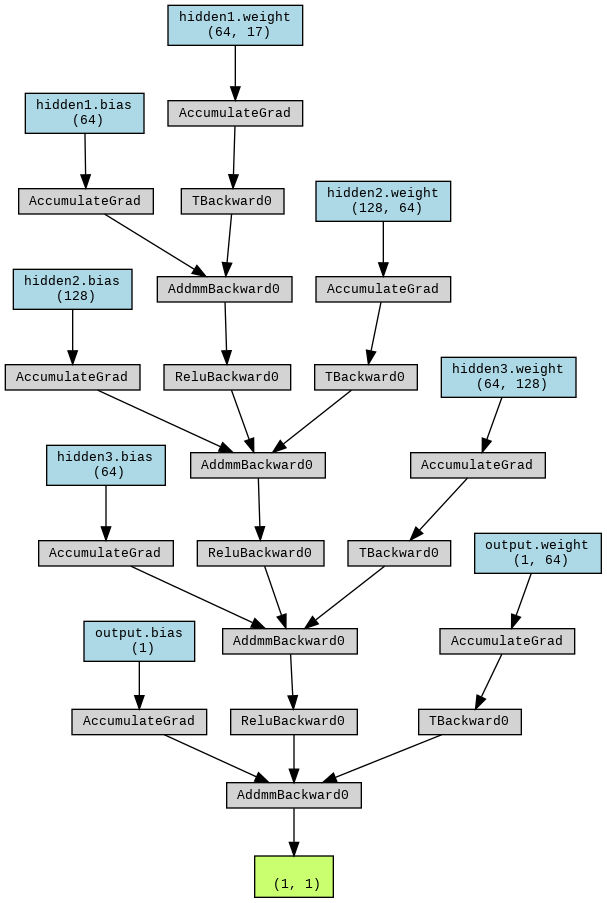
\includegraphics[scale=0.65]{NN}
\centering
\caption{Neural Network architecture}
\label{fig:NN}
\end{figure}

\begin{figure}[H]
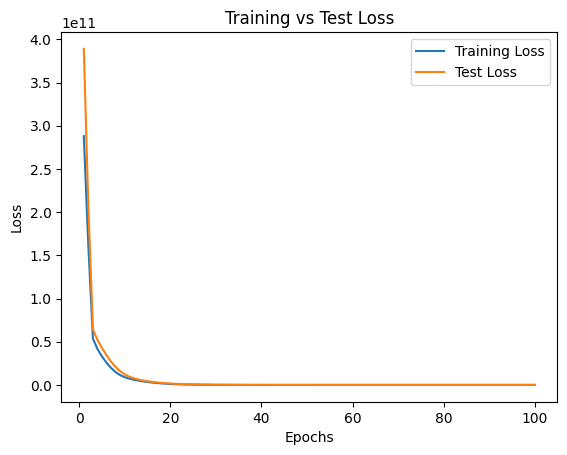
\includegraphics[scale=0.65]{traintestloss}
\centering
\caption{Neural Network training}
\label{fig:traintestloss}
\end{figure}

\begin{figure}[H]
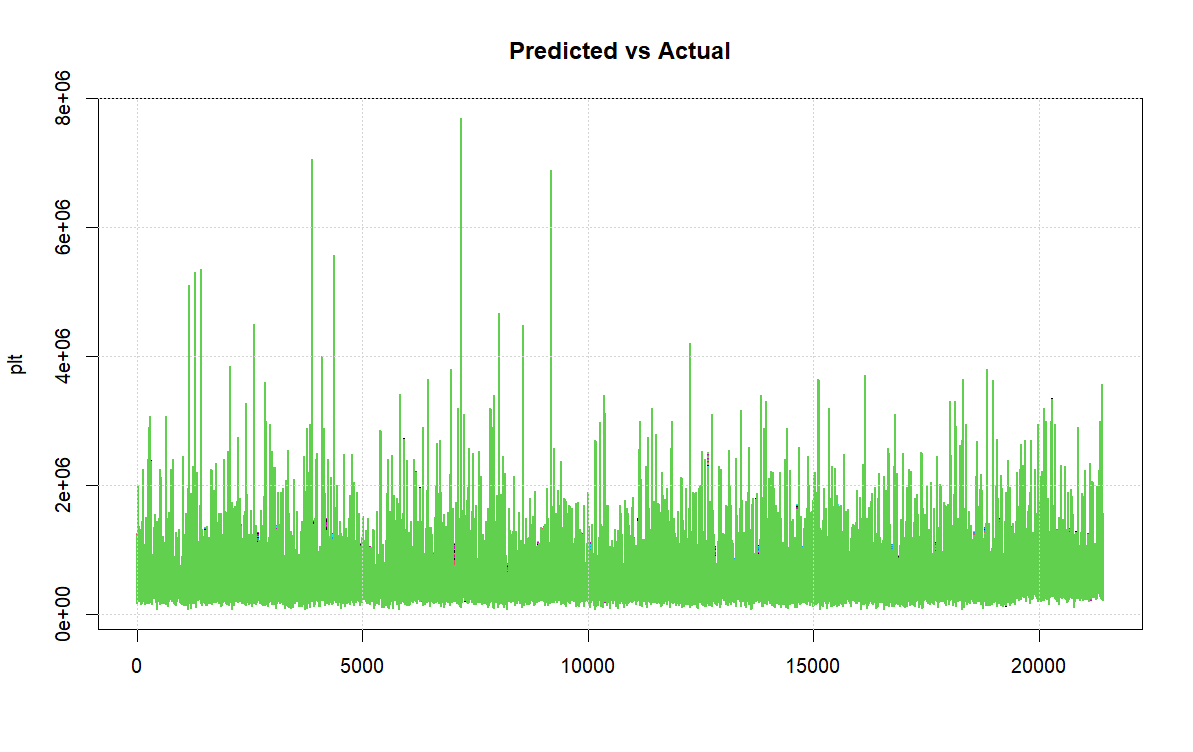
\includegraphics[scale=0.5]{gglasso1pred}
\centering
\caption{Group set 1 actual vs predicted}
\label{fig:gglasso1pred}
\end{figure}

\begin{figure}[H]
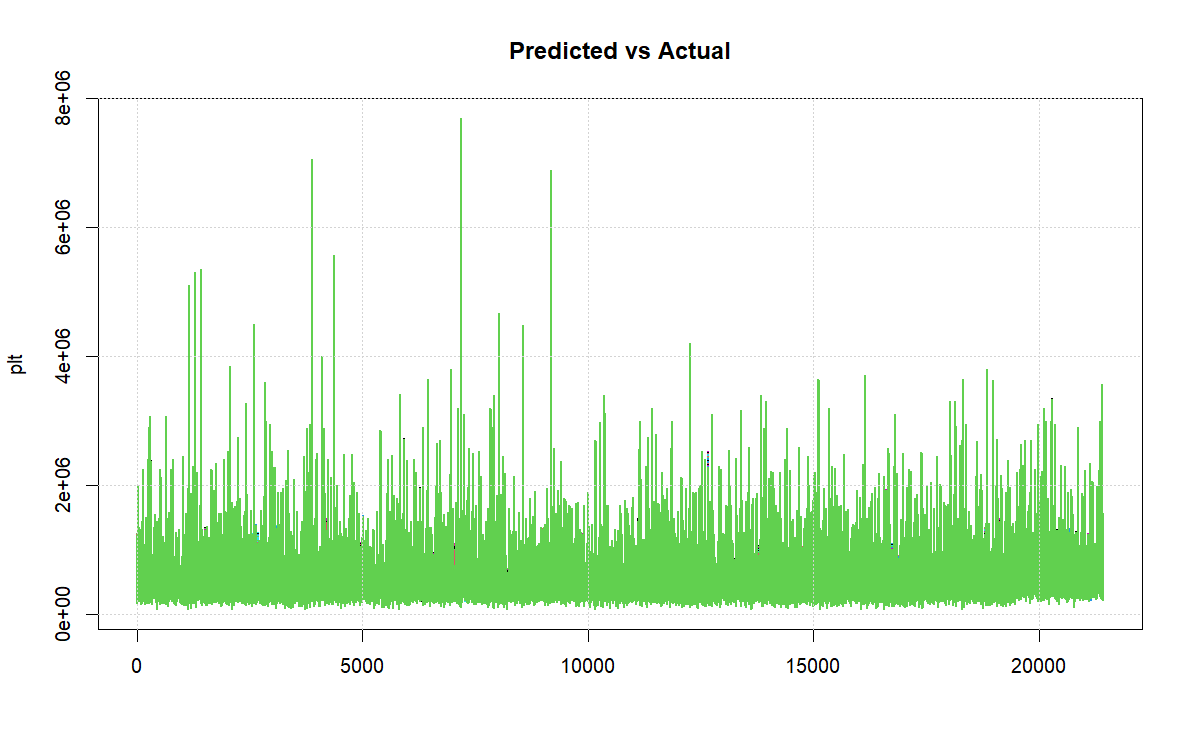
\includegraphics[scale=0.5]{gglasso2pred}
\centering
\caption{Group set 2 actual vs predicted}
\label{fig:gglasso2pred}
\end{figure}

\begin{table}[ht]
\centering
\begin{tabular}{|c|c|c|c|}
\hline
\textbf{Model} & \textbf{MSE} & \textbf{R\(^2\)} & \textbf{MAE} \\
\hline
Model 1 & 13572908807 & -11.50303 & 48891.6 \\
Model 2 & 11156390644 & -9.27699 & 43118.46 \\
\hline
\end{tabular}
\caption{Group Lasso evaluation metrics}
\label{tab:nn}
\end{table}

\begin{figure}[H]
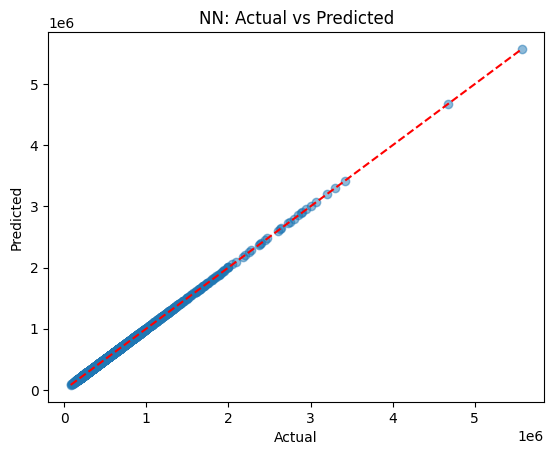
\includegraphics[scale=0.65]{NNpred}
\centering
\caption{Neural Network actual vs predicted}
\label{fig:NNpred}
\end{figure}



\end{document}
